%% slides.tex  –  Schrödinger Bridge / Dynamic OT in 1-D
%% Compile:  pdflatex slides.tex   (twice for TOC)
\documentclass[10pt,aspectratio=169]{beamer}

% ── Theme ──────────────────────────────────────────────────────────────────
\usetheme{Madrid}
\usecolortheme{seahorse}
\setbeamertemplate{navigation symbols}{}
\setbeamertemplate{footline}[frame number]

% ── Packages ───────────────────────────────────────────────────────────────
\usepackage{amsmath,amssymb,mathtools}
\usepackage{booktabs}
\usepackage{multimedia}
\usepackage{tikz}
\usetikzlibrary{arrows.meta,positioning,calc,shapes.geometric}
\usepackage{xcolor}

% ── Macros ─────────────────────────────────────────────────────────────────
\newcommand{\R}{\mathbb{R}}
\newcommand{\eps}{\varepsilon}
\newcommand{\rhoO}{\rho_0}
\newcommand{\rhoT}{\rho_1}
\newcommand{\lx}{\lambda_x}
\newcommand{\lt}{\lambda_t}
% Staggered operators
%   D_t : N_t x (N_t-1)  time derivative  (rho-grid -> phi-grid)
%   I_t : N_t x (N_t-1)  time average     (rho-grid -> phi-grid)
%   D_x : N_x x (N_x-1)  space divergence (m-grid   -> phi-grid)
%   L_x = -D_x D_x^T : Neumann Laplacian (negative semidefinite)
\newcommand{\Dt}{D_t}
\newcommand{\DtT}{D_t^{\!\top}}
\newcommand{\It}{I_t}
\newcommand{\ItT}{I_t^{\!\top}}
\newcommand{\Dx}{D_x}
\newcommand{\DxT}{D_x^{\!\top}}
\newcommand{\Lx}{L_x}
\newcommand{\kron}{\otimes}
% Differential operators (space)
\newcommand{\Lapx}{\Delta_x}          % spatial Laplacian
\newcommand{\Laptx}{\Delta_{t,x}}     % space-time Laplacian  partial_tt + partial_xx
\newcommand{\Bihar}{\Delta_x^2}       % biharmonic (spatial)
\newcommand{\divx}{\nabla_{\!x}\cdot} % spatial divergence
\newcommand{\gradx}{\nabla_{\!x}}     % spatial gradient

\definecolor{myblue}{RGB}{31,119,180}
\definecolor{myred}{RGB}{214,39,40}
\definecolor{mygreen}{RGB}{44,160,44}
\definecolor{warnorange}{RGB}{220,120,0}

\title[SB in 1-D via ADMM]{%
  \textbf{Schr\"{o}dinger Bridge in 1-D via Staggered-Grid ADMM}}
\subtitle{Motivation $\cdot$ Formulation $\cdot$ Discretisation $\cdot$
          Projection Solvers $\cdot$ Stability}
\author{}
\date{\today}

\begin{document}

\begin{frame}
  \titlepage
\end{frame}

\begin{frame}{Outline}
  \tableofcontents
\end{frame}

% ============================================================
\section{Motivation: Why Not Sinkhorn?}
% ============================================================

\begin{frame}{The Two Approaches to Regularised OT}
  \textbf{Same underlying problem}: move mass from $\rhoO$ to $\rhoT$
  at minimum cost, with entropic regularisation $\eps > 0$.

  \bigskip
  \begin{columns}[T]
    \column{0.48\textwidth}
    \textbf{Static / Sinkhorn approach}\\[4pt]
    Solve the $N_x \times N_x$ coupling problem:
    \[
      \min_{\pi \geq 0}\langle C,\pi\rangle + \eps\langle\pi,\log\pi\rangle,
      \quad
      \pi\mathbf{1}=\mathbf{a},\;\pi^\top\mathbf{1}=\mathbf{b}.
    \]
    Solution:
    $\pi^* = \mathrm{diag}(\mathbf{u})\,K\,\mathrm{diag}(\mathbf{v})$,
    \[
      K_{ij} = e^{-C_{ij}/\eps},
      \quad C_{ij} = |x_i - y_j|^2.
    \]
    Sinkhorn iterations: alternating row/column scaling of $K$.

    \column{0.48\textwidth}
    \textbf{Dynamic / Benam\^{o}u--Brenier approach}\\[4pt]
    Solve the space-time PDE-constrained problem on an
    $N_x \times N_t$ grid:
    \[
      \min_{\rho,m}\;\tfrac{1}{2}\iint\frac{m^2}{\rho}
      \quad\text{s.t.}\quad
      \partial_t\rho + \divx m = \eps\,\Lapx\rho.
    \]
    $\eps$ appears as a \emph{PDE diffusion coefficient},
    never inside an exponential.
  \end{columns}

  \bigskip
  \begin{block}{Equivalent as $\eps \to 0$}
    Both formulations share the same $\eps$: as $\eps\to 0$ they recover
    the same unregularised $W_2$ transport.  The key question is what
    happens \emph{numerically} when $\eps$ is small.
  \end{block}
\end{frame}

\begin{frame}{Sinkhorn Breaks Down for Small $\eps$}
  \begin{columns}[T]
    \column{0.52\textwidth}
    \begin{alertblock}{Problem 1: Numerical underflow in $K$}
      $K_{ij} = e^{-C_{ij}/\eps}$ underflows to \texttt{0.0}
      when $C_{ij}/\eps \gtrsim 700$ (IEEE 754 double).

      \smallskip
      Example: $C_{ij} = |x_i - y_j|^2 \sim 0.1$,
      $\eps = 10^{-4}$:
      $K_{ij} = e^{-1000} \approx 0$.

      \smallskip
      Log-domain Sinkhorn helps but adds complexity and
      does not cure the ill-conditioning.
    \end{alertblock}

    \begin{alertblock}{Problem 2: Exponential iteration count}
      Hilbert metric analysis: convergence factor
      $r \approx 1 - 2e^{-\Delta c/\eps} \to 1$ as $\eps\to 0$.

      \smallskip
      Iterations needed: $O(e^{\Delta c/\eps})$ — \textbf{exponential}.

      \smallskip
      For $\Delta c \sim 1$, $\eps = 10^{-3}$: $\sim e^{1000}$ iterations.
    \end{alertblock}

    \column{0.46\textwidth}
    \begin{alertblock}{Problem 3: Dense $N_x^2$ matrix}
      $K$ is $N_x \times N_x$ and dense.
      Each Sinkhorn iteration costs $O(N_x^2)$.
      Total cost $O(N_x^2/\eps)$.

      \smallskip
      No spatial sparsity is exploited.
    \end{alertblock}

    \begin{block}{Dynamic formulation: no exponentials}
      $\eps$ enters the FP equation as a coefficient;
      numerics are independent of $e^{-1/\eps}$.

      \smallskip
      ADMM projection costs $O(N_x N_t\log N_x)$
      per iteration (using DCT and tridiagonal solves).

      \smallskip
      The effective $N$ is the \emph{space-time grid size}
      $N_x N_t$, not the quadratic coupling matrix $N_x^2$.
    \end{block}
  \end{columns}
\end{frame}

\begin{frame}{Sinkhorn Iteration Count Explodes as $\eps \to 0$}
  \vspace{-2pt}
  \begin{center}
    \includegraphics[width=0.82\textwidth,height=0.62\textheight,keepaspectratio]%
      {../../../test/hopfCole/eps_study.png}
  \end{center}
  \vspace{-6pt}
  {\footnotesize
  \textbf{Hopf-Cole Sinkhorn} (1-D/2-D/3-D).
  \textbf{Top}: cold start; \textbf{Bottom}: $\eps$-annealing (8 levels).
  \textcolor{myred}{$\times$} = did not converge within budget (500/4000 iters).
  Iteration count grows \emph{exponentially} as $\eps\!\to\!0$; grid size and
  annealing only shift the curve.  The dynamic BB/ADMM formulation avoids this entirely.}
\end{frame}

% ============================================================
\section{Problem Formulation}
% ============================================================

\begin{frame}{Benam\^{o}u--Brenier and Schr\"{o}dinger Bridge}
  \begin{block}{Dynamic OT}
  \[
    \min_{\rho,m}\;
    \int_0^1\!\int_0^1
    \frac{m(t,x)^2}{2\,\rho(t,x)}\,dx\,dt
    \quad\text{s.t.}\quad
    \underbrace{\partial_t\rho + \divx m = \eps\,\Lapx\rho}_{\text{Fokker--Planck}},\;
    \rho(0,\cdot)=\rhoO,\;\rho(1,\cdot)=\rhoT,\;
    m|_{\partial\Omega}=0.
  \]
  \end{block}

  \begin{itemize}
    \item $\eps = 0$: continuity equation, objective $= W_2(\rhoO,\rhoT)^2$.
    \item $\eps > 0$: Schr\"{o}dinger bridge — most likely diffusion path from
          $\rhoO$ to $\rhoT$ under Brownian motion with diffusivity $\eps$.
    \item \textbf{Gaussian-to-Gaussian exact solution}
          ($\rhoO = \mathcal{N}(\mu_0,\sigma_0^2)$,
           $\rhoT = \mathcal{N}(\mu_1,\sigma_1^2)$):
    \[
      \sigma_{\rm SB}^2(t)
      = (1-t)^2\sigma_0^2
        + 2t(1-t)\sqrt{\eps^2+\sigma_0^2\sigma_1^2}
        + t^2\sigma_1^2.
    \]
  \end{itemize}

  \medskip
  \textbf{ADMM splitting:}
  introduce consensus copy $(\tilde\rho,\bar m)$ constrained to $\mathcal{C}$:
  \[
    \min\;
    \underbrace{f(\rho,m)}_{\text{kinetic energy}}
    + \underbrace{\iota_{\mathcal{C}}(\tilde\rho,\bar m)}_{\text{FP constraint}}
    \quad\text{s.t.}\quad (\rho,m)=(\tilde\rho,\bar m).
  \]
\end{frame}

\begin{frame}{Optimise First or Discretise First?}
  \begin{columns}[T]
    \column{0.48\textwidth}
    \begin{block}{Discretise first, then optimise}
      Discretise the FP constraint on a grid: $A_h(\rho_h,m_h)=0$.
      Run ADMM in the finite-dimensional space.
      Projection $=$ linear solve $(A_hA_h^\top)\phi_h = f_h$.

      \smallskip
      \textbf{Appealing for standard OT} ($\eps=0$):
      $A_m A_m^\top = -\Lapx$, inverted by FFT.
      The matvec $A_h$ is a local stencil --- GPU-friendly.

      \smallskip
      \textbf{Fails for SB} ($\eps>0$): $A_\rho = \partial_t - \eps\Lapx$
      couples space and time.  $A_\rho A_\rho^\top$ involves $\Bihar$;
      no GPU-friendly separable inversion exists.
    \end{block}

    \column{0.48\textwidth}
    \begin{block}{Optimise first, then discretise}
      Derive the projection formula analytically in the
      \emph{continuous} setting, then discretise the result carefully.

      \smallskip
      \textbf{Advantage:} boundary terms and the adjoint structure
      are visible before any discretisation.
      A staggered grid then makes $A_h^\top$ the \emph{exact}
      discrete adjoint of $A_h$.

      \smallskip
      \textbf{Challenge:} even with the correct structure, a naive
      discretisation of the resulting linear system still fails.
    \end{block}
  \end{columns}

  \medskip
  \begin{alertblock}{Our path}
    A discretise-first GPU approach could not be made to work for SB.
    We adopt the \textbf{optimise-first} approach.
  \end{alertblock}
\end{frame}

\begin{frame}{The Continuous Projection Formula: $AA^*\phi = f$}
  Given $(\mu,\psi)$, the ADMM projection step minimises
  $\tfrac{1}{2}\|\rho-\mu\|^2 + \tfrac{1}{2}\|m-\psi\|^2$
  subject to $A_\rho\rho + A_m m = 0$.

  \smallskip
  \textbf{KKT} ($\phi$: Lagrange multiplier):
  $\tilde\rho = \mu - A_\rho^*\phi$,\;
  $\tilde m = \psi - A_m^*\phi$.
  Substituting into the FP constraint gives $AA^*\phi = f$,\;
  $f = A_\rho\mu + A_m\psi$, with
  \[
    A_\rho = \partial_t - \eps\Lapx,\quad
    A_\rho^* = -\partial_t - \eps\Lapx,\quad
    A_m = \divx,\quad
    A_m^* = -\gradx.
  \]
  The $\partial_t\Lapx$ cross-terms cancel, yielding:
  \[
    \boxed{-\Laptx\phi + \eps^2\Bihar\phi = f,}
    \qquad \Laptx = \partial_{tt} + \Lapx.
  \]
  \textbf{Biharmonic-type PDE}: space-time Laplacian $+$ biharmonic in $x$.
  Well-posed with Neumann BCs; for $\eps=0$ reduces to $-\Laptx\phi=f$.

  \smallskip
  \begin{alertblock}{The discretisation challenge}
    A naive (cell-centred, non-staggered) discretisation of this PDE
    satisfies the FP constraint only up to $O(\eps/\Delta t)$ errors.
    For $\eps \gtrsim 10^{-4}$, $\Delta t=1/128$: the projection is
    inaccurate and ADMM \emph{diverges}.
    A staggered grid is required — but even then, the discrete
    normal equations have a non-trivial boundary structure.
  \end{alertblock}
\end{frame}

% ============================================================
\section{Staggered-Grid Discretisation}
% ============================================================

\begin{frame}{Staggered Grid and Operator Notation}
  \begin{columns}[c]
    \column{0.48\textwidth}
    \textbf{Variable locations}:

    \smallskip
    \begin{tabular}{@{}lll@{}}
      \toprule
      Var.& Time & Space \\
      \midrule
      $\rho$ & interior faces & centres \\
             & $(N_t{-}1)\times N_x$ & \\[3pt]
      $m$    & centres & interior faces \\
             & $N_t\times(N_x{-}1)$ & \\
      \bottomrule
    \end{tabular}

    \vspace{8pt}
    \textbf{Four matrix operators}:

    \smallskip
    \begin{tabular}{@{}ll@{}}
      $\Dt\!: N_t{\times}(N_t{-}1)$ & time FD (rho$\to$phi) \\
      $\ItT$, $\ItT\!: (N_t{-}1){\times} N_t$ & time avg (adjoints) \\
      $\Dx\!: N_x{\times}(N_x{-}1)$ & space divergence \\
    \end{tabular}

    \vspace{6pt}
    \textbf{Discrete Laplacian} ($N_x{\times}N_x$, neg.\ semidef.):
    \[
      \Lx = -\Dx\DxT \;\leftrightarrow\; -\Lapx, \quad
      \Lx v_k = -\lx(k)\,v_k.
    \]

    \column{0.50\textwidth}
    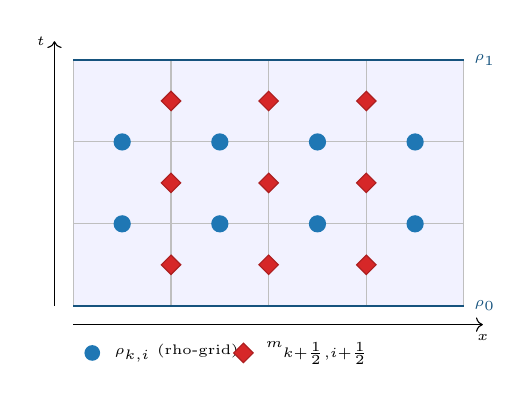
\begin{tikzpicture}[scale=0.80]
      \def\nx{4}\def\nt{3}\def\dx{1.55}\def\dt{1.3}
      \foreach \i in {0,...,2}{\foreach \j in {0,...,3}{
        \fill[blue!5] (\j*\dx,\i*\dt) rectangle (\j*\dx+\dx,\i*\dt+\dt);}}
      \foreach \j in {0,...,4}{\draw[gray!50] (\j*\dx,0)--(\j*\dx,3*\dt);}
      \foreach \i in {0,...,3}{\draw[gray!50] (0,\i*\dt)--(4*\dx,\i*\dt);}
      \foreach \i in {1,...,2}{\foreach \j in {0,...,3}{
        \node[circle,fill=myblue,inner sep=2.2pt]
          at (\j*\dx+0.5*\dx,\i*\dt){};}}
      \foreach \i in {0,...,2}{\foreach \j in {1,...,3}{
        \node[diamond,fill=myred,inner sep=1.8pt,draw=myred!80!black]
          at (\j*\dx,\i*\dt+0.5*\dt){};}}
      \draw[thick,myblue!70!black] (0,0)--(4*\dx,0)
        node[right,font=\tiny]{$\rhoO$};
      \draw[thick,myblue!70!black] (0,3*\dt)--(4*\dx,3*\dt)
        node[right,font=\tiny]{$\rhoT$};
      \draw[->](-0.3,0)--(-0.3,3*\dt+0.3)node[left,font=\tiny]{$t$};
      \draw[->](0,-0.3)--(4*\dx+0.3,-0.3)node[below,font=\tiny]{$x$};
      \node[circle,fill=myblue,inner sep=2pt] at (0.3,-0.75){};
      \node[right,font=\tiny] at (0.5,-0.75){$\rho_{k,i}$\ (rho-grid)};
      \node[diamond,fill=myred,inner sep=1.8pt,draw=myred!80!black]
        at (2.7,-0.75){};
      \node[right,font=\tiny] at (2.9,-0.75){$m_{k+\frac12,i+\frac12}$};
    \end{tikzpicture}

    \vspace{4pt}
    \textbf{DCT diagonalises $\Lx$}:
    \[
      V \Lx V^\top = -\operatorname{diag}(\lx),
      \quad \lx(k) \geq 0.
    \]
    Same for $\Dt\DtT$: time-Neumann Laplacian with
    eigenvalues $\lt(l) \geq 0$.
  \end{columns}
\end{frame}

\begin{frame}{FP Operator as a Kronecker Sum}
  Vectorise $\phi$ column-major ($N_t$ fast) to get
  $\phi_{\rm vec} \in \R^{N_t N_x}$.  Then:

  \[
    A = \bigl[\,A_\rho \;\big|\; A_m\,\bigr],
    \qquad\text{where}
  \]

  \begin{columns}[c]
    \column{0.50\textwidth}
    \begin{block}{Density operator $A_\rho$}
    \[
      \boxed{A_\rho = I_{N_x}\kron \Dt \;+\; \eps\,\Lx\kron\It}
    \]
    \vspace{-4pt}
    \begin{itemize}
      \item $I_{N_x}\kron\Dt$: apply $\Dt$ to every spatial column.
      \item $\eps\,\Lx\kron\It$: average in time \emph{then} apply
            $\Lx$ across space.
    \end{itemize}
    \end{block}

    \column{0.48\textwidth}
    \begin{block}{Momentum operator $A_m$}
    \[
      \boxed{A_m = \Dx\kron I_{N_t}}
    \]
    \vspace{-4pt}
    \begin{itemize}
      \item $\Dx\kron I_{N_t}$: apply space divergence $\Dx$ to
            every time row.
    \end{itemize}
    \end{block}
  \end{columns}

  \bigskip
  \textbf{Adjoint} $A^\top\phi_{\rm vec} = [A_\rho^\top\phi_{\rm vec};\;A_m^\top\phi_{\rm vec}]$:
  \[
    A_\rho^\top = I_{N_x}\kron\DtT + \eps\,\Lx\kron\ItT,
    \qquad
    A_m^\top = \DxT\kron I_{N_t}.
  \]
  These are used in the projection update:
  $(\rho_{\rm out}, m_{\rm out}) = (\mu,\psi) - A^\top\phi$.
\end{frame}

\begin{frame}{Normal Equations via Kronecker Algebra}
  The projection solves $(AA^\top)\phi = f$.
  Expand using $(A\kron B)(C\kron D) = AC\kron BD$:

  \smallskip
  \begin{align*}
    A_\rho A_\rho^\top
    &= (I\kron\Dt)(I\kron\DtT)
     + \eps\,({\Lx}\kron\Dt\ItT + \Lx\kron\It\DtT)
     + \eps^2\,\Lx^2\kron\It\ItT \\
    &= I\kron\Dt\DtT
     + \eps\,\Lx\kron\underbrace{(\Dt\ItT+\It\DtT)}_{\text{rank-2!}}
     + \eps^2\,\Lx^2\kron\It\ItT, \\[4pt]
    A_m A_m^\top
    &= (\Dx\kron I)(\DxT\kron I)
     = \underbrace{\Dx\DxT}_{=-\Lx}\kron I
     = -\Lx\kron I.
  \end{align*}

  \medskip
  \begin{alertblock}{The rank-2 boundary identity}
  \[
    \Dt\ItT + \It\DtT
    = \frac{1}{\Delta t}\bigl(e_1 e_1^\top - e_{N_t}e_{N_t}^\top\bigr)
    \quad\text{(proved by direct computation)}.
  \]
  \end{alertblock}

  \smallskip
  Substituting and collecting:
  \[
    AA^\top
    = \underbrace{I\kron\Dt\DtT - \Lx\kron I + \eps^2\Lx^2\kron\It\ItT}_{\widetilde{P}\ (\It\ItT\text{ not circulant — corrected next slide})}
    \;+\;
    \underbrace{\frac{\eps}{\Delta t}\,\Lx\kron(e_1 e_1^\top - e_{N_t}e_{N_t}^\top)}_{E\ (\mathrm{rank\text{-}}2\text{ in }t)}.
  \]
\end{frame}

\begin{frame}{The $\It\ItT$ Boundary Error — and Its Rank-2 Structure}
  $\It\ItT$ has interior diagonal $\tfrac{1}{2}$ but \textbf{corner entries $\tfrac{1}{4}$}.
  Splitting off the circulant (periodic-BC) part $(\It\ItT)_{\rm circ}$ with
  eigenvalues $\sigma_t(l)=\cos^2(\pi l\Delta t/2)$:
  \[
    \It\ItT
    = \underbrace{(\It\ItT)_{\rm circ}}_{\text{DCT-diagonalisable}}
      \;-\;
      \underbrace{\tfrac{1}{4}\bigl(e_1 e_1^\top + e_{N_t}e_{N_t}^\top\bigr)}_{E_2\ (\text{rank-2!})}.
  \]

  \smallskip
  So the full $AA^\top$ splits into a \emph{circulant} base plus
  \textbf{two} rank-2 boundary corrections:
  \[
    AA^\top
    = \underbrace{I\kron\Dt\DtT - \Lx\kron I
        + \eps^2\Lx^2\kron(\It\ItT)_{\rm circ}}_{P_{\rm circ}\text{ (exact 2-D DCT)}}
    +\;
    \underbrace{\frac{\eps}{\Delta t}\Lx\kron(e_1 e_1^\top - e_{N_t}e_{N_t}^\top)}_{E}
    \;-\;
    \underbrace{\frac{\eps^2}{4}\Lx^2\kron(e_1 e_1^\top + e_{N_t}e_{N_t}^\top)}_{E_2}.
  \]

  \begin{block}{Woodbury can handle both $E$ and $E_2$}
    In DCT-$x$ mode $k$, the combined correction is
    \[
      F_k = \Bigl(-\tfrac{\eps\lx}{\Delta t} - \tfrac{\eps^2\lx^2}{4}\Bigr)\,e_1 e_1^\top
            + \Bigl(\tfrac{\eps\lx}{\Delta t} - \tfrac{\eps^2\lx^2}{4}\Bigr)\,e_{N_t}e_{N_t}^\top.
    \]
    Both $E$ and $E_2$ involve only $e_1,e_{N_t}$, so $F_k$ is still
    \textbf{rank-2 in time} — the same $2{\times}2$ Woodbury system, extended
    coefficients. The extended Woodbury is then \emph{exactly} correct.
  \end{block}
\end{frame}

% ============================================================
\section{The Naive Approach: Why It Fails}
% ============================================================

\begin{frame}{Why Every Naive Discretisation Fails}
  Even with a correct staggered grid, the first (ad-hoc) projection
  ignored the rank-2 correction $E$: it solved $P_{\rm DCT}\,\phi = f$
  via a plain 2-D DCT.

  \medskip
  \begin{alertblock}{Root cause: the rank-2 boundary term $E$ is dropped}
    $AA^\top = P_{\rm DCT} + E$ but the solver treats it as $P_{\rm DCT}$,
    leaving a systematic residual
    \[
      \|AA^\top\phi - f\| \;\approx\; \|E\phi\|
      \;=\; \frac{\eps}{\Delta t}\|\Lx\|\cdot|\phi(1)-\phi(N_t)|.
    \]
    For $\eps=10^{-4}$, $\Delta t=1/128$:\ $\eps/\Delta t=0.013$ — already
    noticeable.  The FP constraint is not satisfied at any grid cell.
    For $\eps \gtrsim 10^{-4}$ ADMM \emph{diverges}.
  \end{alertblock}

  \begin{block}{Why does ADMM stagnate / diverge?}
    The returned $(\rho,m)$ satisfies a \emph{wrong} normal equation.
    The constraint residual stalls at $O(\eps/\Delta t)$ regardless of
    iteration count.  Larger $\eps$ makes the violation proportionally worse.
  \end{block}

  \smallskip
  \textbf{Fix:} include \emph{all} boundary corrections ($E$ and $E_2$)
  in the solve — either via the extended Woodbury or the banded solver.
\end{frame}

% ============================================================
\section{Woodbury Projection (Approximate)}
% ============================================================

\begin{frame}{Woodbury: Correcting the Rank-2 Boundary Terms}
  \textbf{Setup.} After DCT-$x$, mode $k$ decouples. We must solve
  \[
    \bigl(P_{{\rm circ},k} + F_k\bigr)\phi_k = f_k,
    \quad
    F_k = \alpha_k\,e_1 e_1^\top + \beta_k\,e_{N_t}e_{N_t}^\top,
  \]
  where $P_{{\rm circ},k}$ is \emph{diagonal in DCT-$t$} and $F_k$ is \textbf{rank-2}.
  The coefficients combining both boundary corrections $E$ and $E_2$ are:
  \[
    \alpha_k = -\tfrac{\eps\lx(k)}{\Delta t} - \tfrac{\eps^2\lx(k)^2}{4},
    \qquad
    \beta_k  = \phantom{-}\tfrac{\eps\lx(k)}{\Delta t} - \tfrac{\eps^2\lx(k)^2}{4}.
  \]

  \textbf{Woodbury identity.} With $U=[e_1,e_{N_t}]$ and $C=\operatorname{diag}(\alpha_k,\beta_k)$:
  \[
    (P_{{\rm circ},k}+F_k)^{-1}f_k
    = \underbrace{P_{{\rm circ},k}^{-1}f_k}_{g_k}
      - P_{{\rm circ},k}^{-1}U\,M_k^{-1}\,U^\top g_k,
  \]
  where $M_k = C^{-1} + U^\top P_{{\rm circ},k}^{-1}U$ is a \textbf{precomputed $2{\times}2$ matrix}.

  \textbf{Algorithm per mode $k$:}
  \begin{enumerate}
    \item $g_k = P_{{\rm circ},k}^{-1}f_k$:\; DCT-$t$, divide by $P_{\rm circ}$ eigenvalues, IDCT-$t$.
    \item Extract boundary values $c_k = [g_k(1);\,g_k(N_t)]$.
    \item Solve $2{\times}2$ system: $[a_k;\,b_k] = M_k^{-1}c_k$.
    \item $\phi_k = g_k - a_k\,d_{1,k} - b_k\,d_{N_t,k}$,\quad
          where $d_{j,k} = P_{{\rm circ},k}^{-1}e_j$ (precomputed).
  \end{enumerate}
  Steps 1--4 cost $O(N_t\log N_t)$ per mode $\Rightarrow$ $O(N_xN_t\log N_t)$ total.
\end{frame}

\begin{frame}{Woodbury Stability: $2{\times}2$ Condition Number}
  \begin{columns}[T]
    \column{0.54\textwidth}
    The dominant correction coefficient grows with $\eps$ and frequency:
    \[
      |\alpha_k|,|\beta_k| \;\sim\; \frac{\eps\,\lx(k)}{\Delta t}
          \;\approx\; \frac{\eps\,k^2}{\Delta x^2\,\Delta t}.
    \]
    For high modes $k\sim N_x$:
    \[
      |\alpha_k| \;\sim\; \frac{\eps\,N_x^2\,N_t}{1}.
    \]
    \textbf{Condition number of $M_k$:}
    $\kappa(M_k) = O(|\alpha_k|^2).$

    This amplifies rounding errors in $[a_k;b_k]$,
    corrupting $\phi$ for high spatial modes.

    \column{0.44\textwidth}
    \begin{exampleblock}{$N_x=128$, $\Delta t=1/128$, $\eps=0.1$}
      $|c_{N_x}| \approx 0.1\times 128^2\times 128 \approx 2\times10^5$\\
      $\kappa(M_{N_x}) \sim 4\times10^{10}$\\[4pt]
      IEEE double: 16 significant digits.\\
      $\Rightarrow$ $\phi$ accurate to $\sim6$ digits.\\
      Projection residual $\sim10^{-6}$, not $\sim10^{-14}$.
    \end{exampleblock}

    \begin{alertblock}{Summary}
      Woodbury is exact in exact arithmetic; in floating point, the
      $2{\times}2$ condition number grows as
      $O(\eps^2 N_x^4 N_t^2)$.
    \end{alertblock}
  \end{columns}
\end{frame}

\begin{frame}{Woodbury Results: $N_x{=}N_t{=}128$, $\eps{=}10^{-2}$, $\gamma{=}1$}
  \begin{columns}[T]
    \column{0.50\textwidth}
    \textbf{Convergence} (successive difference $\|u_{k+1}-u_k\|$):
    \medskip

    \includegraphics[width=\linewidth]%
      {../figures/gaussian/nx128_nt128_gamma1_eps1e-2_woodbury/convergence.pdf}

    \column{0.48\textwidth}
    \textbf{Density transport animation}:
    \medskip

    \movie[externalviewer,width=\linewidth,height=0.55\linewidth]%
      {\includegraphics[width=\linewidth]%
        {../figures/gaussian/nx128_nt128_gamma1_eps1e-2_woodbury/convergence.pdf}}%
      {../figures/gaussian/nx128_nt128_gamma1_eps1e-2_woodbury/transport.mp4}

    \vspace{4pt}
    {\footnotesize Click image above to play \texttt{transport.mp4} in external player.}

    \smallskip
    \begin{alertblock}{\small Note}
      {\small Woodbury corrects $E$ only ($P_{\rm circ}$ approximates $\It\ItT$).
      Works at $\eps{=}10^{-2}$; degrades for larger $\eps$ as $\kappa(M_k)$ grows.}
    \end{alertblock}
  \end{columns}
\end{frame}

% ============================================================
\section{Banded Projection (Exact and Stable)}
% ============================================================

\begin{frame}{Banded Solver: Block-Diagonalise Only in $x$}
  Apply DCT only in $x$ (diagonalise $\Lx\to-\lx(k)$).
  The Kronecker structure $I_{N_x}\kron(\cdot)$ vs $\Lx\kron(\cdot)$
  decouples into $N_x$ independent $N_t{\times}N_t$ systems.

  \medskip
  \textbf{Mode-$k$ operator} (obtained by substituting $\Lx\to-\lx(k)$ in $A_\rho$):
  \[
    A_{\rho,k} = \Dt - \eps\,\lx(k)\,\It,
    \qquad
    (A_m A_m^\top)_k = \lx(k)\,I_{N_t}.
  \]

  \medskip
  \textbf{Per-mode normal equation:}
  \[
    T_k\,\hat\phi_k = \hat f_k,
    \qquad
    \boxed{T_k = A_{\rho,k}A_{\rho,k}^\top + \lx(k)\,I_{N_t}}.
  \]

  \medskip
  \textbf{Expanding} $A_{\rho,k}A_{\rho,k}^\top$ and using
  $\Dt\ItT + \It\DtT = \frac{1}{\Delta t}(e_1 e_1^\top - e_{N_t}e_{N_t}^\top)$:
  \begin{align*}
    T_k
    &= \Dt\DtT
     - \eps\lx(k)\underbrace{(\Dt\ItT+\It\DtT)}_{=\,\frac{1}{\Delta t}(e_1e_1^\top - e_{N_t}e_{N_t}^\top)}
     + \eps^2\lx(k)^2\,\It\ItT
     + \lx(k)\,I \\[4pt]
    &= \underbrace{\Dt\DtT}_{M_0}
     + \lx(k)\underbrace{\operatorname{diag}\!\bigl(1{-}\tfrac{\eps}{\Delta t},1,\ldots,1,1{+}\tfrac{\eps}{\Delta t}\bigr)}_{M_1}
     + \lx(k)^2\underbrace{\eps^2\It\ItT}_{M_2}.
  \end{align*}
\end{frame}

\begin{frame}{Banded Solver: Algorithm, DC Mode, and Stability}
  \textbf{$M_0$, $M_1$, $M_2$ are all tridiagonal or diagonal
  $\Rightarrow$ $T_k$ is tridiagonal. Solved in $O(N_t)$ per mode.}

  \medskip
  \textbf{Per-call algorithm:}
  \begin{enumerate}
    \item DCT in $x$ of $f=A(\mu,\psi)$: cost $O(N_xN_t\log N_x)$.
    \item For $k\geq 2$: tridiagonal solve $\hat\phi_k = T_k^{-1}\hat f_k$.
          Cost $O(N_xN_t)$ total.
    \item \textbf{Special case $k=1$} ($\lx(1)=0$, so $T_1 = M_0 = \Dt\DtT$, singular):
    \[
      \hat\phi_1(l) = \begin{cases}0 & l=1\text{ (gauge fix)},\\
      \hat f_1(l)\,/\,\lt(l) & l\geq 2.\end{cases}
      \quad\text{(DCT-}t\text{ solve, cost }O(N_t\log N_t))
    \]
    \item IDCT in $x$; apply $A^\top = [I\kron\DtT + \eps\Lx\kron\ItT;\;\DxT\kron I]$.
  \end{enumerate}

  \medskip
  \begin{alertblock}{Bug if $k=1$ is skipped}
    ADMM iterates have non-constant total mass; $\hat f_1$ has nonzero
    non-DC-in-$t$ components. Setting $\hat\phi_1=0$ leaves these permanently,
    causing stagnation for all $\eps$.
  \end{alertblock}

  \medskip
  \begin{block}{Stability: $\kappa(T_k) = O(N_t^2/\lx(k))$, independent of $\eps$}
    Since $T_k = A_{\rho,k}A_{\rho,k}^\top + \lx(k)I \succeq \lx(k)I$,
    the minimum eigenvalue is $\lx(k)>0$ regardless of $\eps$.
  \end{block}
\end{frame}

\begin{frame}{Banded Results: $N_x{=}N_t{=}128$, $\eps{=}10^{-2}$, $\gamma{=}1$}
  \begin{columns}[T]
    \column{0.50\textwidth}
    \textbf{Convergence} (successive difference $\|u_{k+1}-u_k\|$):
    \medskip

    \includegraphics[width=\linewidth]%
      {../figures/gaussian/nx128_nt128_gamma1_eps1e-2_banded/convergence.pdf}

    \column{0.48\textwidth}
    \textbf{Density transport animation}:
    \medskip

    \movie[externalviewer,width=\linewidth,height=0.55\linewidth]%
      {\includegraphics[width=\linewidth]%
        {../figures/gaussian/nx128_nt128_gamma1_eps1e-2_banded/convergence.pdf}}%
      {../figures/gaussian/nx128_nt128_gamma1_eps1e-2_banded/transport.mp4}

    \vspace{4pt}
    {\footnotesize Click image above to play \texttt{transport.mp4} in external player.}

    \smallskip
    \begin{exampleblock}{\small Stability}
      {\small $\kappa(T_k) = O(N_t^2/\lx(k))$, \emph{independent of $\eps$}.
      Exact solve — no floating-point amplification.}
    \end{exampleblock}
  \end{columns}
\end{frame}

% ============================================================
\section{PCG Projection}
% ============================================================

\begin{frame}{PCG: Exact Matvec, Approximate Preconditioner}
  \texttt{sb1d\_admm\_pcg.m}: preconditioner $M{=}P_{\rm circ}$ (ignores $E,E_2$);
  exact matvec $AA^\top\phi$; 30 inner CG iterations per ADMM step.

  \smallskip
  \begin{columns}[T]
    \column{0.54\textwidth}
    \begin{alertblock}{Why $O(N_x)$ CG iterations are needed}
      $E = \frac\eps{\Delta t}\Lx\kron(e_1 e_1^\top{-}e_{N_t}e_{N_t}^\top)$
      has \textbf{rank $2(N_x{-}1)$} in the full space
      ($\mathrm{rank}(\Lx){=}N_x{-}1$,\ $\mathrm{rank}(e_1e_1^\top{-}e_{N_t}e_{N_t}^\top){=}2$).
      $P_{\rm circ}^{-1}AA^\top$ has $O(N_x)$ eigenvalues off from~1;
      CG needs $O(N_x)$ extra iterations to deflate them.

      \smallskip
      $N_x{=}128$, 30-iteration cap: only $\sim\!23\%$ of outliers
      handled.  CG \emph{stalls}; projection is inaccurate;
      ADMM diverges.
    \end{alertblock}

    \column{0.43\textwidth}
    \begin{block}{Outlier eigenvalue}
      At the DC time mode ($\lt{=}0$), mode $k$:
      \[
        \mu_{1,k} \approx 1 - \frac{\eps/\Delta t}{1+\eps^2\lx(k)}.
      \]
      Largest at $k{=}2$: $\approx 1{-}\eps/\Delta t$.

      \smallskip
      \textbf{For $\eps>\Delta t$}: $\mu_{1,k}<0$, system is
      \emph{indefinite}.  CG triggers \texttt{pAp}${\leq}0$
      failure and exits with bad $\phi$.
    \end{block}

    \begin{exampleblock}{Banded solver wins}
      Exact, $O(N_t)$ per mode, no iteration count tuning.
    \end{exampleblock}
  \end{columns}
\end{frame}

% ============================================================
\section{Comparison}
% ============================================================

\begin{frame}{Four Projection Methods: Side-by-Side}
  \renewcommand{\arraystretch}{1.3}
  \begin{center}
  {\footnotesize
  \begin{tabular}{@{}lcccc@{}}
    \toprule
    & \textbf{Naive} & \textbf{Woodbury} & \textbf{PCG} & \textbf{Banded} \\
    \midrule
    Exact?
      & {\color{myred}No}
      & {\color{mygreen}Yes}
      & {\color{warnorange}If converged}
      & {\color{mygreen}Yes} \\
    Handles $E,E_2$?
      & {\color{myred}No}
      & {\color{mygreen}Yes}
      & {\color{warnorange}Via matvec}
      & {\color{mygreen}Yes} \\
    Large-$\eps$ behaviour
      & {\color{myred}Diverges}
      & {\color{warnorange}$\kappa\!\sim\!\eps^2N_x^4N_t^2$}
      & {\color{myred}Stalls/$-$PD}
      & {\color{mygreen}Stable} \\
    Failure mode
      & Missing $E$
      & Ill-cond.\ $2{\times}2$
      & $O(N_x)$ iters needed
      & None \\
    \midrule
    Cost/call
      & $O(N^2\!\log N)$
      & $O(N^2\!\log N)$
      & $O(k_{\rm CG}N^2)$
      & $O(N^2\!\log N_x)$ \\
    Precomp.
      & $O(N^2)$
      & $O(N^2\!\log N_t)$
      & $O(N^2)$
      & $O(N^2)$ \\
    \bottomrule
  \end{tabular}}
  \end{center}

  \smallskip
  \textbf{Recommendation}: \textbf{banded solver} for all $\eps$
  (\texttt{opts.proj\_method = 'banded'}).
\end{frame}

\begin{frame}{Key Takeaways}
  \begin{enumerate}
    \setlength\itemsep{5pt}
    \item \textbf{Optimise first.}
          Deriving the continuous projection formula $AA^*\phi=f$
          (a 4th-order PDE) first, then discretising, reveals the correct
          adjoint structure.  A GPU-friendly discretise-first approach could
          not be made to work for the SB diffusion coupling.

    \item \textbf{Dynamic OT avoids Sinkhorn's $e^{-c/\eps}$ blow-up.}
          Same $\eps$; no exponentially small numbers in the dynamic formulation.

    \item \textbf{Kronecker structure}
          $A_\rho = I\kron\Dt + \eps\Lx\kron\It$,\ $A_m = \Dx\kron I$
          makes the algebra transparent and immediately reveals the $P_{\rm circ}+E+E_2$ split.

    \item \textbf{Two rank-2 boundary terms} ($E$ and $E_2$) arise from
          the staggered grid.  Ignoring either causes ADMM to stall at
          $O(\eps/\Delta t)$ constraint violation regardless of iteration count.

    \item \textbf{Extended Woodbury} corrects $E$+$E_2$ exactly via
          $\alpha_k,\beta_k$, but the $2{\times}2$ condition number grows as
          $O(\eps^2 N_x^4 N_t^2)$ — unstable for large $\eps$.

    \item \textbf{PCG} uses an exact matvec but an approximate preconditioner.
          The un-preconditioned correction $E$ has rank $O(N_x)$ in the full
          space, requiring $O(N_x)$ CG iterations.  With a 30-iteration cap,
          PCG stalls for $\eps/\Delta t \not\ll 1$; for $\eps>\Delta t$ the
          preconditioned system is indefinite and CG loses positive definiteness.

    \item \textbf{Banded solver}: exact, $O(N_xN_t\log N_x)$, $\eps$-stable.
          Strictly superior to all alternatives.
  \end{enumerate}
\end{frame}

\end{document}
